\chapter{Desarrollo de la Web}
\label{desarrolloWeb}
\section{Introducci'on}

Internet es una red de interconexi'on global de redes individuales alrededor del mundo. Originalmente fu'e utilizada para interconectar laboratorios dedicados a la investigaci'on gubernamental. Desde 1994 se expandi'o para millones de usuarios de todo el mundo que la utilizan con m'ultiples prop'ositos. A medida que fu'e creciendo, cambi'o la forma de hacer negocios y de comunicarse hasta llegar a ser una fuente de informaci'on universal para millones de personas \citep{iws}.

\section{El crecimiento de Internet}

Internet es un medio que sigue creciendo de manera exponencial. Hacia 1995 la cantidad de usuarios promedio era de 16 millones, 1 a'no despu'es, la cifra ascendi'o a m'as del doble. Para el a'no 2000 se increment'o 10 veces la cantidad de usuarios. Esta informaci'on puede verse en el Cuadro \ref{cuadroCrecInternet}.

\begin{longtable}{l c c}
\hline
 Fecha & Usuarios(mill) & \% Poblaci'on Mundial\\
\hline \hline
\endfirsthead

\hline
 Fecha & Usuarios(mill) & \% Poblaci'on Mundial\\
\hline \hline
\endhead

\multicolumn{3}{l}{Sigue en la p'agina siguiente.}
\endfoot

\endlastfoot

\hline
Diciembre, 1995 & 16 & 0.4 \\
Diciembre, 1996 & 36 & 0.9 \\
Diciembre, 1997 & 70 & 1.7 \\
Diciembre, 1998 & 147 & 3.6 \\
Diciembre, 1999 & 248 & 4.1 \\
Diciembre, 2000 & 361 & 5.8 \\
Agosto, 2001 & 513 & 8.6 \\
Septiembre, 2002 & 587 & 9.4 \\
Diciembre,  2003 & 719 & 11.1 \\
Diciembre,  2004 & 817 & 12.7 \\
Diciembre,  2005 & 1018 & 15.7 \\
Diciembre, 2006 & 1093 & 16.7 \\
Diciembre, 2007 & 1319 & 20.0 \\
Diciembre, 2008 & 1574 & 23.5 \\
Marzo, 2009 & 1596 & 23.8 \\
Junio, 2009 & 1669 & 24.7 \\
Septiembre, 2009 & 1734 & 25.6 \\
Diciembre, 2009 & 1802 & 26.6 \\
Junio, 2010 & 1966 & 28.7 \\
Septiembre, 2010 & 1971 & 28.8 \\
Marzo, 2011 & 2095 & 30.2 \\
Junio, 2011 & 2110 & 30.4 \\
Septiembre, 2011 & 2180 & 31.5 \\
Diciembre, 2011 & 2267 & 32.7 \\
Marzo, 2012 & 2336 & 33.3 \\
Junio, 2012 & 2405 & 34.3 \\
Septiembre, 2012 & 2439 & 34.8 \\
Diciembre, 2012 & 2497 & 35.7 \\
Marzo, 2013 & 2749 & 38.8 \\
\hline
\caption{Crecimiento de la cantidad de usuarios de Internet, informaci'on extra'ida de \cite{iws}}
\label{cuadroCrecInternet}
\end{longtable}

Tambi'en puede observarse en el Gr'afico \ref{grafCrecInternet} el crecimiento exponencial que tuvo la cantidad de usuarios de Internet, y es clara la tendencia de seguir creciendo.

\begin{figure}[h]
  	\centering
	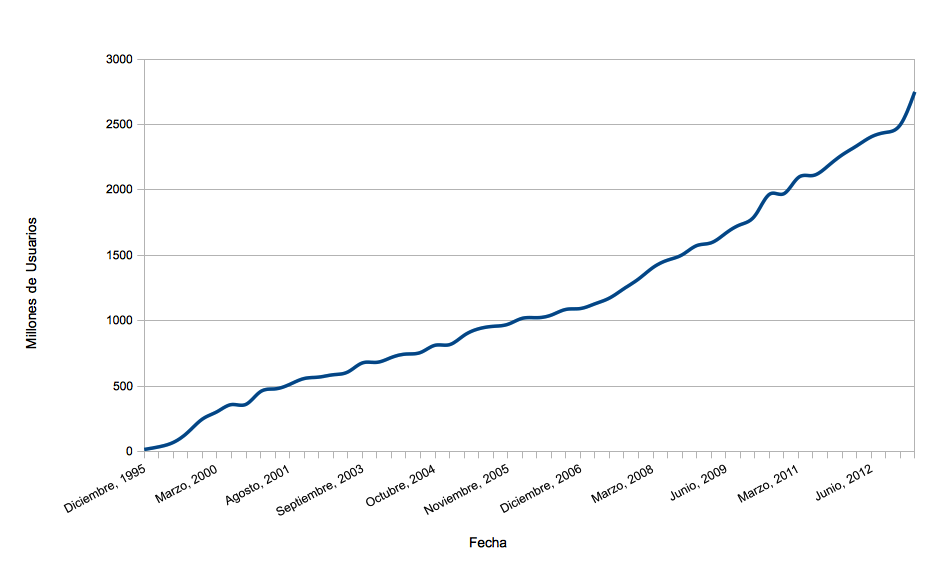
\includegraphics[width=\textwidth]{img/grafCrecInternet}
	\caption{\small Crecimiento de la cantidad de usuarios de Internet, informaci'on extra'ida de \cite{iws}}
	\label{grafCrecInternet}
\end{figure}

Adem'as de la cantidad de usuarios, en paralelo iba creciendo la cantidad de dominios\footnote{Nombre que identifica un sitio web, se asocia a una direcci'on IP (ver \ref{tcpip}) 'unica.}. En sus inicios, la cantidad de dominios era de 19.732 (medici'on realizada en Agosto de 1995), la medici'on m'as actual (Febrero 2014) realizada por Netcraft\footnote{NetCraft - http://news.netcraft.com/} da un total aproximado de sitios de 920.102.079 \citep{netcraft} (58 millones m'as que el mes anterior). Esto se puede ver en el Gr'afico \ref{grafNetcraft}.

\begin{figure}[h]
  	\centering
	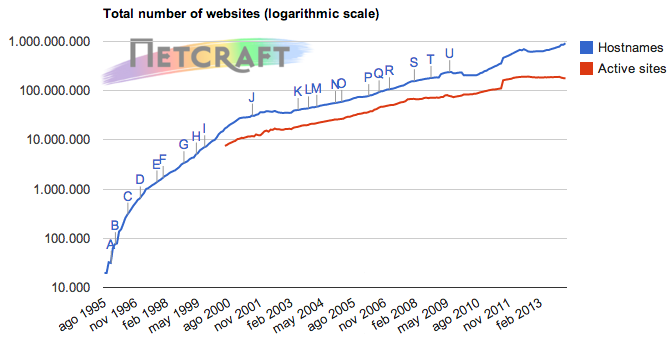
\includegraphics[width=\textwidth]{img/grafNetcraft}
	\caption{\small Crecimiento de la cantidad de sitios en Internet, extra'ido de \cite{netcraft}}
	\label{grafNetcraft}
\end{figure}

\section{El crecimiento de los sitios}

Se define sitio como el conjunto de p'aginas relacionadas, que se encuentran en un servidor web, bajo un mismo dominio en Internet. El aumento del tama'no promedio de los sitios as'i tambi'en como la cantidad de recursos que poseen los mismos, es otra variable que entra en juego.

En el a'no 1997, el tama'no promedio de un sitio era de 60Kb \citep{atw}, pr'acticamente era todo texto, pocas im'agenes y poca interactividad. Esto fu'e cambiando con el tiempo, con el avance de la tecnolog'ia y de los recursos que se pod'ian compartir en la red. El crecimiento a lo largo del tiempo puede verse en el Gr'afico \ref{grafCrecSitios}.

\begin{figure}[ht!]
  	\centering
	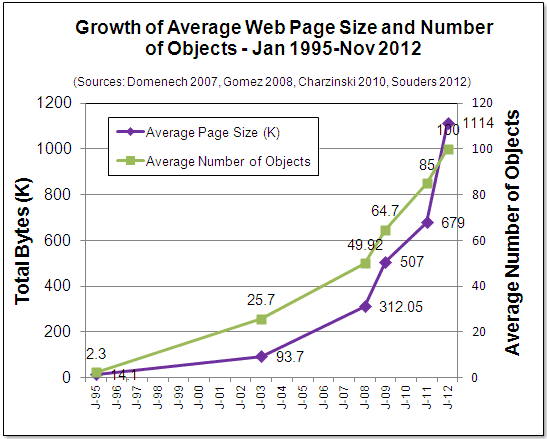
\includegraphics[width=300px]{img/grafCrecSitios}
	\caption{\small Crecimiento del tama'no de los sitios en Internet (1995 a 2012), extra'ido de \cite{tamanoSitios}}
	\label{grafCrecSitios}
\end{figure}

Hoy en d'ia, el contenido de los sitios es mucho m'as variado e interactivo. Se componen de diversos tipos de recursos: scripts, hojas de estilo, variados tipos de im'agenes, video, contenido Flash\footnote{http://www.adobe.com/}, etc. Esto produce un aumento en el tiempo de carga de las p'aginas y la necesidad de poseer un dispositivo con la capacidad necesaria para procesarla y renderizarla\footnote{El navegador "dibuja" la p'agina seg'un el c'odigo HTML y el estilo.}.

Comparando 2 medidas realizadas por HTTP Archive\citep{httparchive}  con casi 4 a'nos de diferencia, se observa que, en la primera medici'on el promedio es de 702Kb\footnote{Medici'on extra'ida de \citep{httparchive} el 15 de Noviembre de 2010.}, el promedio detallado por contenido de los sitios se puede ver en el Gr'afico \ref{grafSitios2010}. En la segunda medici'on realizada en Junio de 2014, se observa que el promedio es de 1808Kb, es decir, que hubo un aumento de un 157\%.

\begin{figure}[h]
  	\centering
	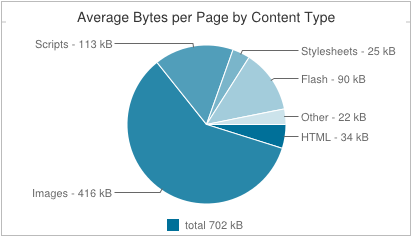
\includegraphics[width=300px]{img/grafSitios2010}
	\caption{\small Tama'no promedio de los sitios en Internet (Noviembre 2010), detallado por contenido, extra'ido de \cite{httparchive}}
	\label{grafSitios2010}
\end{figure}

\begin{figure}[h]
  	\centering
	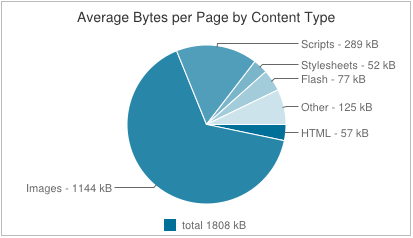
\includegraphics[width=300px]{img/grafSitios2014}
	\caption{\small Tama'no promedio de los sitios en Internet (Junio 2014), detallado por contenido, extra'ido de \cite{httparchive}}
	\label{grafSitios2014}
\end{figure}

Otra cuesti'on es el aumento de la utilizaci'on de HTTPS\footnote{Hypertext Transfer Protocol Secure.}, la versi'on segura de HTTP (ver Cap'itulo \ref{protocolos}), como se ver'a m'as adelante, este protocolo a'nade tiempo en la negociaci'on previa a recuperar la p'agina.

\begin{figure}[h]
  	\centering
	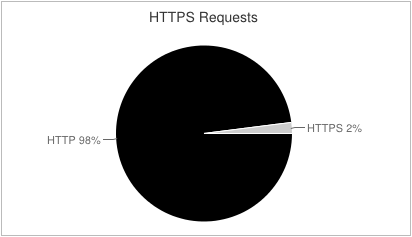
\includegraphics[width=300px]{img/httphttps2010}
	\caption{\small Porcentaje de utilizaci'on de HTTP/HTTPS (Noviembre 2010), extra'ido de \cite{httparchive}}
	\label{httphttps2010}
\end{figure}

\begin{figure}[h]
  	\centering
	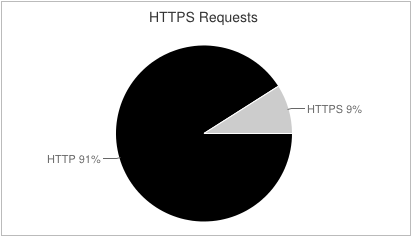
\includegraphics[width=300px]{img/httphttps2014}
	\caption{\small Porcentaje de utilizaci'on de HTTP/HTTPS (Junio 2014), extra'ido de \cite{httparchive}}
	\label{httphttps2014}
\end{figure}

El aumento de complejidad de los sitios, hace que el protocolo HTTP, que originalmente fu'e dise'nado para p'aginas ''simples'', baje su performance, aumentando el tiempo de carga de las p'aginas. No fu'e especialmente dise'nado para latencia, la demanda actual de la web no se pudo haber previsto cuando se desarroll'o. Esto motiva a repensar el protocolo, y revisar cuestiones como: petici'on individual por conexi'on, peticiones iniciadas exclusivamente por los clientes, headers de petici'on y respuesta sin compresi'on, headers redundantes, compresi'on opcional. Estas caracter'isticas y otras se ver'an en el Cap'itulo siguiente.